\chapter{Código para realizar la integración COMPSs+OmpSs-2}
\label{appendix:integration}

\section{Ejecutar tareas de COMPSs como tareas de OmpSs-2}

Para la implementación de los \textit{workers} hay dos ficheros distintos \textit{nio\_worker\_c.cc} y \textit{worker\_c.cc} respectivamente para el persistente y el no persistente. En cada uno de estos ficheros deberemos añadir el código para que cuando los compilemos con la opción de \textit{OmpSs-2} y \textit{COMPSs} los ejecute (en función de si es persistente o no) y activen el modo librería.

\bigskip

\begin{minipage}{\linewidth}
\begin{lstlisting} [caption={Código necesario para la gestión del modo librería de Nanos6 en nio\_worker\_c.cc y worker\_c.cc},captionpos=b, label={lst:managementnanosworkers}, language=C++]

#ifdef OMPSS2_ENABLED
#include <pthread.h>
#include <nanos6/bootstrap.h>
#include <nanos6/library-mode.h>
#endif

    ...

#ifdef OMPSS2_ENABLED
    char const *error = nanos6_library_mode_init();
    if (error != NULL)
    {
        fprintf(stderr, "Error initializing Nanos6: %s\n", error);
        return 1;
    }
    std::cout << "[C-BINDING] Nanos6 initialized" << std::endl;
#endif

    ...
    
#ifdef OMPSS2_ENABLED
    nanos6_shutdown();
    std::cout << "[C-BINDING] Nanos6 shutdown" << std::endl;
#endif

\end{lstlisting}
\end{minipage}

\par\bigskip

El código mostrado en la imagen \ref{lst:managementnanosworkers} se divide en tres bloques divididos por puntos suspensivos, el código que hubiera entre estos, depende de si el fichero es \textit{nio\_worker\_c.cc} o \textit{worker\_c.cc} y es independiente de ellos. Se hace uso de macros del preprocesador de \textit{C}, la macro \textit{\#ifdef VAR} comprueba en tiempo de compilación si la variable \textit{OMPSS2\_ENABLED} está definida, si lo está las líneas contenidas entre la primera y el \textit{\#endif} serán incluidas en el fichero, sino no lo serán.
\par\medskip
En cuánto a los tres bloques, el primero incluye cabeceras necesarias para \textit{Nanos6}, y el resto han sido ya explicados en la sección \ref{spawnfunction}.
\par\bigskip

En el caso de \textit{OmpSs}, hay que registrar exactamente los \textit{threads} de un proceso que ejecutarán tareas y también hay que compilar necesariamente toda la aplicación con \textit{Mercurium} y el \textit{flag} \textit{-{}-ompss}, pero por otra parte, no hay necesidad de añadir más código a parte del que se encarga de registrar los \textit{threads}. En \textit{OmpSs-2} como vimos en el ejemplo, es necesario hacer una gestión más compleja en cuánto a generación de código, pero es independiente del \textit{thread} en el cuál se ejecuta.
\par\bigskip
Con tal de cambiar el código que se genera en el \textit{executor}, hay que hacer modificaciones en el programa que compila la interfaz del programa para generar el \textit{stubs}, el \textit{executor} y el resto de ficheros necesarios. En la estructura que tenemos nosotros del compilador, el fichero que contiene el código para autogenerarlo todo es \textit{c-backend.c}, en el cuál deberemos hacer unas modificaciones.
\par\smallskip
Vamos a centrarnos en las modificaciones que harán que podamos generar el \textit{struct} personalizado para cada tarea y la llamada a \textit{nanos6\_spawn\_function}, pero cómo se genera el mecanismo de sincronización  (\textit{pthread\_cond\_wait}, \textit{pthread\_cond\_signal} y las estructuras de datos necesarias) es trivial, ya que no varía según la aplicación que se compile, es siempre el mismo.
\par\bigskip
Con tal de generar el \textit{struct} para cada tarea, incluiremos su definición en los ficheros que hacen la función de cabecera. Cada \textit{struct} será único para cada tarea (podría tener los mismos campos, pero nunca el mismo nombre). Para generar el \textit{struct} de la tarea, necesitamos tener información sobre la función que se ejecutará, contamos con una estructura \textit{function} que almacena toda la información necesaria.
\par\bigskip

La imagen \ref{lst:structs} contiene el código necesario para incluir en la cabecera la definición del \textit{struct} de una función en concreto. Se recorrerán los argumentos de la función y se comprobará si tiene retorno, habrá un campo del \textit{struct} por cada argumento que tenga la función y uno adicional en caso de que tenga retorno.

\bigskip

\begin{minipage}{\linewidth}
\begin{lstlisting} [caption={Función para generar la definición de los structs.},captionpos=b, label={lst:structs}, language=C++]
static void generate_struct_nanos6_wrapper(FILE *outFile, 
Types current_types,
function *func) {
argument *arg;
fprintf(outFile, "typedef struct {\n", func->methodname);

char* return_type = construct_returntype(func);

if (func->return_type != void_dt && return_type != NULL) {
fprintf(outFile, "\t% s ret;\n", return_type);
}

arg = func->first_argument;
while (arg != NULL) {
fprintf(outFile, "\t% s;\n", construct_type_and_name(arg));
arg = arg->next_argument;
}
fprintf(outFile, "} % s_struct_t;\n", func->methodname);
}
\end{lstlisting}
\end{minipage}

\par\bigskip
Para generar el código del \textit{wrapper} lo primero que necesitamos hacer es generar el nombre de la función, que es del estilo ''function\_wrapper'' y tiene por argumento un puntero a \textit{void} que apunta al \textit{struct} que contiene los argumentos para la función que vamos a ejecutar y el valor de retorno de esta en caso que tenga. Entonces, si la función tiene retorno distinto del tipo \textit{void}, la ejecutaremos asignándole el valor al \textit{struct}, en caso contrario tan sólo la ejecutaremos, si algún valor de los argumentos se modifica, la única posibilidad para que esto se refleje en \textit{COMPSs} es que fuera un puntero, por lo que quedará modificado también dentro del \textit{struct}.

\smallskip
La imagen \ref{lst:wrapper} muestra como está hecho.
\bigskip

%\begin{minipage}{\linewidth}
\begin{lstlisting} [caption={Función para generar el wrapper de la tarea.},captionpos=b, label={lst:wrapper}, language=C++]

static void generate_nanos6_wrapper(FILE *outFile, function* func) {
fprintf(outFile, "void % s_wrapper(void* args) {\n", 
func->methodname);

fprintf(outFile, 
"\t% s_struct_t* struct_ = (% s_struct_t*) args;\n", 
func->methodname, 
func->methodname);

char* func_to_execute;
int printed_chars = 0;

if (func->return_type != NULL && func->return_type != void_dt) {
fprintf(outFile, "\tstruct_->ret = ", func->return_type);
}

if ((func->classname != NULL) && (func->access_static == 0)) {
printed_chars = asprintf(&func_to_execute, 
"\t% s->% s(", 
func->name, 
func->methodname);
} else {
printed_chars = asprintf(&func_to_execute, 
"\t% s(", func->name);
}

if (printed_chars < 0) {
asprintf_error(func_to_execute, 
"ERROR: Not possible to 
generate method execution.\n");
}

fprintf(outFile, "% s", func_to_execute);

argument* args = func->first_argument;

int first = 1;
while (args != NULL) {
if (first) {
first = 0;
}
else {
fprintf(outFile, ", ");
}
fprintf(outFile, "struct_->% s", args->name);

args = args->next_argument;
}

fprintf(outFile, ");\n");
fprintf(outFile, "}\n");
}  
\end{lstlisting}
%end{minipage}
\par\bigskip

Ahora ya tenemos lo que necesitamos, \textit{structs} para pasar los argumentos, el \textit{wrapper} del que haremos \textit{spawn} y la propia tarea que se acabará ejecutando, tan sólo falta hacer la llamada a \textit{nanos6\_spawn\_function}. Para hacer esto, tenemos que declarar el \textit{struct} y asignarle los valores que vienen de \textit{COMPSs}, acto seguido se generará la llamada a \textit{nanos6\_spawn\_function} con el \textit{wrapper} como función a ejecutar desde \textit{OmpSs-2}, la dirección del \textit{struct} que contiene los argumentos y todo lo necesario para efectuar los mecanismos de sincronización que vimos en la sección \ref{sec:mecanismosync}. Una vez hemos esperado a que la tarea se haya ejecutado, si el retorno era distinto del tipo \textit{void} hay que asignarlo al retorno de la tarea a nivel de \textit{COMPSs}. En la imagen \ref{lst:spawncompss} se ve el código que se encarga de generar esta parte.
\bigskip

\begin{minipage}{\linewidth}
\begin{lstlisting} [caption={Código para hacer un spawn de una tarea para OmpSs-2 en COMPSs.},captionpos=b, label={lst:spawncompss}, language=C++]
fprintf(outFile, "\t\t\t% s_struct_t % s_struct;\n", func->methodname, 
func->methodname);

assign_arguments_to_struct(outFile, func);

char* nanos6_spawner;
printed_chars = asprintf(&nanos6_spawner, 
"\t\t\tnanos6_spawn_function(% s_wrapper,
&% s_struct, 
% s, % s, 
\"% s_spawned_task\");\n",
func->methodname, 
func->methodname, 
"condition_variable_callback", 
"&cond_var", 
func->methodname);

if (printed_chars < 0) {
asprintf_error(nanos6_spawner, 
"Not possible to generate function spawn.\n");
}

fprintf(outFile, "% s\n", nanos6_spawner);

fprintf(outFile, "\t\t\twait_condition_variable(&cond_var);\n");

if (func->return_type != void_dt && func->return_type != NULL) {
char* return_var;
printed_chars = asprintf(&return_var, 
"return_obj = % s_struct.ret;\n", 
func->methodname);

fprintf(outFile, "% s", return_var);

if (printed_chars < 0) {
asprintf_error(return_var, 
"Not possible to generate return variable.\n");
}
}
\end{lstlisting}
\end{minipage}

\bigskip
\section{Entorno de compilado para COMPSs+OmpSs-2}

Para compilar una aplicación que utilice \textit{OmpSs} se necesita poner el \textit{flag} \textit{-{}-ompss} en \textit{Mercurium}, y el \textit{flag} \textit{-{}-ompss-2} para \textit{OmpSs-2}. En la anterior integración se compilaba la totalidad de los ficheros con \textit{Mercurium} y el \textit{flag} \textit{-{}-ompss} debido a que no existía el modo librería. Ahora, es estrictamente necesario compilar con \textit{Mercurium} y el \textit{flag} \textit{-{}-ompss-2} tan sólo un único fichero, el que contiene las funciones a ejecutar como tareas. 
\par\bigskip
Habrá que modificar el método actual de compilación de una aplicación del \textit{binding} de \textit{C/C++} con tal de que aplique lo relativo a la compilación explicado en la sección \ref{sec:compilado}. Para el usuario compilar una aplicación con \textit{OmpSs} es muy sencillo, ejecutando en el terminal el comando \textit{compss\_build\_app -{}-ompss ejemplo} empezaría el proceso de compilado del \textit{master} y el \textit{worker} de manera automática, en la nueva integración no puede ser más difícil. Antes de indagar en las modificaciones en concreto en los \textit{scripts} vamos a ver una descripción superficial de cómo se hace actualmente.

\bigskip
\begin{figure}[h]
	\centering 
	\caption{Estructura superficial de los \textit{scripts} para compilar una aplicación de COMPSs.}
	%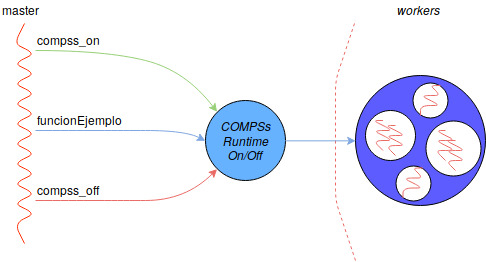
\includegraphics[width=\textwidth]{sta-masterworker.jpg}
	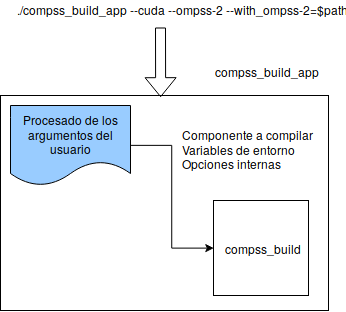
\includegraphics[scale=0.7]{compilation.png}
	\label{fig:compilado}
\end{figure}
\par\bigskip

En la imagen \ref{fig:compilado} vemos que existen dos \textit{scripts}, \textit{compss\_build\_app} y \textit{compss\_build}, el primero es el encargado de recoger los argumentos que el usuario haya introducido para la compilación de su aplicación (si se utiliza \textit{OmpSs}, donde está la instalación de \textit{OmpSs}, si se utiliza \textit{OpenCL}, o \textit{Cuda}, etc) y procesarlos configurando el entorno correcto para la compilación según estos argumentos que ha introducido el usuario. Una vez configurado el entorno se ejecuta el segundo \textit{script} \textit{compss\_build} tanto para el \textit{master} como para el \textit{worker}, que será realmente quién efectúe la compilación. 
\par\bigskip
Para ello se utiliza un conjunto de herramientas muy populares desarrolladas por \textit{GNU},  \textit{Autotools} \ref{appendix:autotools}. Estas herramientas tienen como objetivo facilitar a los usuarios (que no a los desarrolladores...) la compilación y portabilidad entre plataformas. Pese a que es un campo interesante y muy útil, no entraremos demasiado en detalles, daremos una visión general y entraremos en las modificaciones que se han realizado con tal de poder compilar aplicaciones del tipo \textit{COMPSs+OmpSs-2}. 
\par\bigskip
Como ya hemos visto, \textit{compss\_build\_app} hace de alguna manera de \textit{wrapper} de \textit{compss\_build}, es decir, lo ejecuta con los parámetros adecuados las veces que sea necesario. Este segundo, es el que toca de primera mano \textit{Autotools}, con tal de utilizarlo para compilar una aplicación hay que generar una serie de ficheros. La siguiente imagen nos muestra una porción del \textit{script}  \textit{compss\_build} para generar el \textit{script} \textit{autogen.sh}, que al ser ejecutado nos generará estos ficheros que \textit{Autotools} necesita.
\bigskip

\begin{minipage}{\linewidth}
\begin{lstlisting} [caption={Porción del script autogen.sh que genera los ficheros base necesarios para Autotools.},captionpos=b, label={lst:aclocal}, language=bash]
/bin/cat > autogen.sh << EOF
#!/bin/bash
set -e

/usr/bin/aclocal
/usr/bin/automake -a -c
/usr/bin/autoconf
EOF       
\end{lstlisting}
\end{minipage}

\par\bigskip

La primera y la última línea de la imagen \ref{lst:aclocal} sirven para escribir el código contenido entre estas en el fichero \textit{autogen.sh}. El \textit{script} \textit{autogen.sh} es generado por \textit{compss\_build} cada vez que se quiere compilar una aplicación y también en función de si se está compilando el \textit{master} o el \textit{worker} (de hecho, se encuentran en sitios distintos), tendrá una forma u otra. 
\par\smallskip

Una vez ejecutada esta porción del \textit{script} \textit{autogen.sh}, entre otros, esto nos habrá generado un \textit{script} \textit{configure}, que al ser ejecutado generará un \textit{Makefile} adaptado al entorno que hayamos especificado. Nuestro proceso de compilado requiere ser flexible, ya que permitimos utilizar \textit{OmpSs}, a veces con \textit{Cuda}, a veces con \textit{OpenCL}... Por tanto, necesitamos pasarle al compilador dónde se encuentran las librerías que necesitamos, \textit{flags} adicionales que necesitemos (\textit{-{}-ompss}, \textit{-{}-ompss-2}, \textit{-{}-cuda}...). Por suerte, este \textit{configure}, nos permite pasar variables de entorno a tener en cuenta durante la compilación, además de opciones personalizadas, a continuación del código de la imagen \ref{lst:aclocal} añadiremos código para que \textit{autogen.sh} ejecute el \textit{script} \textit{configure} con las opciones que necesitamos.
\bigskip

\begin{minipage}{\linewidth}
\begin{lstlisting} [caption={Porción del script autogen.sh que se encarga de customizar la ejecución de configure.},captionpos=b, label={lst:customconfigure}, language=bash]                                                                                                                                               
if [ "$OMPSS2_ENABLED" == "enabled" ]; then
ldflags_aux="$ldflags_aux -L$OMPSS2_DIR/lib
-Wl,-rpath,$OMPSS2_DIR/lib"
cflags_aux="$cflags_aux -I$OMPSS2_DIR/include"
conf_opts="--with-ompss-2"
fi

if [ "$OMPSS_ENABLED" == "enabled" ]; then
ldflags_aux="$ldflags_aux -L$OMPSS_DIR/lib"
cflags_aux="$cflags_aux -I$OMPSS_DIR/include"
conf_opts="$conf_opts --with-ompss"
fi

if [ "$CUDA_ENABLED" == "enabled" ]; then
ldflags_aux="$ldflags_aux -L$CUDA_HOME/lib64"
cflags_aux="$cflags_aux -I$CUDA_HOME/include"
conf_opts="$conf_opts --with-cuda"
fi

/bin/cat >> autogen.sh << EOF
./configure --with-cs-prefix=$CS_HOME $conf_opts \ 
CXXFLAGS="$CXXFLAGS $cflags_aux"     \  
CFLAGS="$CFLAGS $cflags_aux"         \
LDFLAGS="$LDFLAGS $ldflags_aux" 
EOF

/bin/chmod +x autogen.sh
\end{lstlisting}
\end{minipage}

Anteriormente hemos mencionado que el \textit{script} \textit{compss\_build\_app} es el encargado de recolectar los \textit{flags} que nos interesan del usuario en el proceso de compilación y servirlos al \textit{script} \textit{compss\_build}, como se puede ver en la imagen \ref{lst:customconfigure} en función de si las variables de entorno \textit{OMPSS2\_ENABLED}, \textit{OMPSS\_ENABLED}, o \textit{CUDA\_ENABLED} tienen por valor la cadena de carácteres \textit{enabled}, definirá el valor de los \textit{flags} para la fase de compilación \textit{CXXFLAGS} y \textit{CFLAGS}, que se asignarán via la variable \textit{cflags\_aux} y para la fase de \textit{linking} \textit{LDFLAGS} que se asignará via la variable \textit{ldflags\_aux}, además de las opciones personalizadas (que serán pasadas mediante la variable \textit{conf\_opts}).

\par

Dos ficheros esenciales en todo este proceso, son \textit{configure.ac} y \textit{Makefile.am}, uno utiliza una serie de \textit{macros} para generar de manera customizada \textit{configure} (por ejemplo, con las opciones mencionadas anteriormente), y el otro indica cuáles son los ficheros que deben ser compilados, cómo y adónde irán una vez compilados. Las modificaciones que explicamos ahora mismo sólo se han aplicado al \textit{worker}, para el \textit{master} no se ha necesitado ningún tipo de modificación. Para declarar una opción personalizada en \textit{configure} se utiliza la macro \textit{AC\_ARG\_WITH}, que tiene como argumentos el nombre de la opción (ompss, que pasará a ser with-ompss), el mensaje de ayuda para el usuario y lo que hay que hacer en caso que se habilite la opción, la imagen \ref{lst:ac-ompss} muestra exactamente cómo se hace.

%\begin{minipage}{\linewidth}
\begin{lstlisting} [caption={Macros necesarias en configure.ac para habilitar la opcion --ompss en configure.},captionpos=b, label={lst:ac-ompss}, language=bash]
AC_ARG_WITH([ompss],
AS_HELP_STRING([ --with-ompss], [Enables the use of OmpSs and 
specificates its directory.]),
[
ompss=true
]
)
\end{lstlisting}
%\end{minipage}

\todo{Crec que el tema de que el codi no ocupi mes de una pagina si es possible fa aixo}

Para el resto de opciones se utiliza el mismo mecanismo, pero las acciones a realizar si se habilita la opción son distintas. Con tal de compilar una aplicación de \textit{OmpSs-2} necesitamos librerías de \textit{Pthreads}, \textit{dl}\footnote{https://en.wikipedia.org/wiki/Dynamic\_loading}, \textit{nanos6} (evidentemente para todo lo que concierne al \textit{runtime}), y \textit{custom-nanos6}, que no es más que la adaptación a librería del \textit{nanos6-library-mode.o} que se utilizó en la sección \ref{sec:compilado}. La imagen \ref{lst:ac-ompss-2} muestra exactamente cómo lo hacemos.

\begin{minipage}{\linewidth}
\begin{lstlisting} [caption={Macros necesarias en configure.ac para habilitar la opcion --ompss-2 en configure.},captionpos=b, label={lst:ac-ompss-2}, language=bash]
AC_ARG_WITH([ompss-2],
AS_HELP_STRING([ --with-ompss-2], [Enables the use of OmpSs2 
and specificates its 
directory.]),
[
ompss2=true

AC_CHECK_LIB([pthread], 
[pthread_cond_signal], 
[],
[
AC_MSG_ERROR([Pthread library not found, 
is needed to enable OmpSs2.])
])

AC_CHECK_LIB([dl], 
[dlopen], 
[],
[
AC_MSG_ERROR([dl library not found, 
is needed to enable OmpSs2.])
])

AC_CHECK_LIB([nanos6], 
[nanos6_spawn_function], 
[],
[
AC_MSG_ERROR([Nanos6 library not found, 
is needed to enable OmpSs2.])
])

AC_CHECK_LIB([custom-nanos6], 
[nanos6_library_mode_init], 
[],
[
AC_MSG_ERROR([nanos6-library-mode.o is needed, 
we make a custom library from it.])
])
]
)
\end{lstlisting}
\end{minipage}

\bigskip

En este caso a parte de la macro \textit{AC\_ARG\_WITH} se utiliza \textit{AC\_CHECK\_LIB}, esta macro hará que se compruebe si la librería del primer argumento existe y contiene la función del segundo argumento, el tercer y el cuarto argumento indican respectivamente que se hará si se encuentra la librería y que se hará en caso que no se encuentre. Nótese que esta macro, añade la librería a la variable de entorno \textit{LIBS} (librerías que tomarán parte en la fase de \textit{linking}). En el caso de cuda debemos buscar la librería del \textit{runtime} de \textit{Cuda}, que es \textit{cudart}. Se utilizan exactamente los mismos mecanismos que en el resto de opciones, se muestra exactamente en la imagen \ref{lst:ac-cuda}.

\bigskip

\begin{minipage}{\linewidth}
\begin{lstlisting} [caption={Macros necesarias en configure.ac para habilitar la opcion --cuda en configure.},captionpos=b, label={lst:ac-cuda}, language=bash]
AC_ARG_WITH([cuda],
AS_HELP_STRING([ --with-cuda], [Enables the use of CUDA.]),
[
cuda=true

AC_CHECK_LIB([cudart], 
[cudaMalloc], 
[],
[
AC_MSG_ERROR([cudart library not found, 
is needed to enable CUDA.])
])
]
)
\end{lstlisting}
\end{minipage}

\bigskip

Para todas las opciones, en las imágenes \ref{lst:ac-ompss}, \ref{lst:ac-ompss-2} y \ref{lst:ac-cuda} se asigna el valor a una variable ompss, ompss-2 y cuda respectivamente para cada opción al valor \textit{true}. Con la macro \textit{AC\_CONDITIONAL} asignamos a una variable con el nombre del primer argumento el valor que obtengamos del segundo. Estas variables son visibles en el fichero \textit{Makefile.am}, de manera que podremos condicionar la compilación en función de que opciones pase el usuario al \textit{script} \textit{configure}.

\bigskip

\begin{minipage}{\linewidth}
\begin{lstlisting} [caption={Creación de las variables para el Makefile.am.},captionpos=b, label={lst:ac-vars}, language=bash]
AM_CONDITIONAL([OMPSS]      , [test x$ompss = xtrue])
AM_CONDITIONAL([OMPSS2]     , [test x$ompss2 = xtrue])
AM_CONDITIONAL([CUDAOMPSS]  , [test x$cuda = xtrue && 
test x$ompss = xtrue])
AM_CONDITIONAL([CUDAOMPSS2] , [test x$cuda = xtrue && 
test x$ompss2 = xtrue])
\end{lstlisting}
\end{minipage}

\bigskip

Esto sería todo lo relacionado con el \textit{configure.ac}, ahora entraríamos con el \textit{Makefile.am}. Recordemos que lo único que necesitamos compilar con \textit{-{}-ompss-2} es el fichero que contiene las funciones a ser ejecutadas como tareas, por lo tanto necesitamos hacer una distinción de los \textit{flags} que se utilizan para compilar este fichero. Para conseguir esto, hemos decidido indicar en el \textit{Makefile.am} que se haga una librería de este fichero y se compile con unos \textit{flags} en especial, para así aislarlo del resto. En la siguiente imagen se muestra como se hace esto.

\par\bigskip

La primera línea indica que \textit{libfunctions.a} es una librería que no debe ser instalada, y la segunda que el fichero fuente de esta librería es \textit{PACKAGE-functions.cc} donde \textit{PACKAGE} es el nombre del paquete. Las siguientes líneas indican los \textit{flags} base que se utilizarán para compilar los ficheros fuente.
 
\bigskip

\begin{minipage}{\linewidth}
\begin{lstlisting} [caption={Crear una librería en el Makefile.am.},captionpos=b, label={lst:am-lib}, language=bash]
noinst_LIBRARIES = libfunctions.a
libfunctions_a_SOURCES = PACKAGE-functions.cc

libfunctions_a_CPPFLAGS =  -I../../src -I../../include
-Wno-write-strings -I$(JAVA_HOME)/include 
-I$(JAVA_HOME)/include/linux/ -Wall
-I$(CS_HOME)/../bindings-common/include
-I$(CS_HOME)/include 

libfunctions_a_CFLAGS =
\end{lstlisting}
\end{minipage}

\bigskip

A esta altura, ya tenemos la base para compilar la librería, pero si no podemos poner los \textit{flags} para \textit{OmpSs-2} o \textit{OmpSs} no habremos conseguido nada. Utilizaremos las variables que hemos definido anteriormente en \ref{lst:ac-vars}. Sencillamente, en función de si las variables correspondientes tienen el valor adecuado, añadimos a las variables adecuadas los \textit{flags} que requerimos. Por ejemplo, si el usuario está compilando con \textit{OmpSs-2}, los \textit{flags} para compilar \textit{libfunctions.a} deben contener \textit{-{}-ompss-2} entre otros. En la imagen \ref{lst:am-cond-flags} se procede a asignar los \textit{flags} de esta manera.

\bigskip

\begin{minipage}{\linewidth}
\begin{lstlisting} [caption={Flags de manera condicional en Makefile.am.},captionpos=b, label={lst:am-cond-flags}, language=bash]
if OMPSS2
libfunctions_a_CPPFLAGS  += --ompss-2 -DOMPSS2_ENABLED
libfunctions_a_CFLAGS    += --ompss-2 -DOMPSS2_ENABLED

nio_worker_c_CPPFLAGS    += -DOMPSS2_ENABLED
worker_c_CPPFLAGS        += -DOMPSS2_ENABLED
endif

if OMPSS
libfunctions_a_CPPFLAGS  += --ompss -DOMPSS_ENABLED
libfunctions_a_CFLAGS    += --ompss -DOMPSS_ENABLED

nio_worker_c_CPPFLAGS    += --ompss -DOMPSS_ENABLED
worker_c_CPPFLAGS        += --ompss -DOMPSS_ENABLED

nio_worker_c_LDFLAGS += --ompss
worker_c_LDFLAGS     += --ompss
endif

if CUDAOMPSS
libfunctions_a_CPPFLAGS  += --cuda -DCUDA_ENABLED
libfunctions_a_CFLAGS    += --cuda -DCUDA_ENABLED

nio_worker_c_CPPFLAGS    += --cuda -DCUDA_ENABLED
worker_c_CPPFLAGS        += --cuda -DCUDA_ENABLED

nio_worker_c_LDFLAGS += --cuda
worker_c_LDFLAGS     += --cuda
endif

if CUDAOMPSS2
libfunctions_a_CPPFLAGS  += --cuda -DCUDA_ENABLED
libfunctions_a_CFLAGS    += --cuda -DCUDA_ENABLED
endif
\end{lstlisting}
\end{minipage}

\bigskip

Está claro que después de haber compilado la librería habrá que hacer el \textit{linking} de ella con \textit{nio\_worker\_c} o \textit{worker\_c}. Con esto ya habríamos hecho las modificaciones necesarias para poder compilar la aplicación de \textit{COMPSs+OmpSs-2}.

\section{Soporte para el tipo enum y cabeceras en la interfaz}

Un requisito ha sido soportar el tipo \textit{enum} y añadir la posibilidad de incluir cabeceras en la interfaz de una aplicación \textit{C/C++}. Para hacer esto, ha habido que hacer modificaciones en la gramática del compilador y en la generación de código. Este añadido puede ser muy útil para cuando se utilicen librerías externas en la interfaz y se precise de cabeceras adicionales que incluyan tipos que se necesitan.

\par\bigskip

El compilador está hecho con las herramientas \textit{Lex} (un generador de analizadores léxicos) y \textit{Yacc} (un generador de analizadores sintácticos), es decir, las dos piezas fundamentales para hacer un compilador, ya que uno nos facilitará el reconocimiento de \textit{tokens} en la interfaz y el otro nos permite comprobar que realmente tiene sentido la interfaz y le otorga una semántica.

\par\bigskip

Para añadir el tipo \textit{enum}, la gramática tiene que reconocer algo del estilo "\textit{in/out enum} tipo nombre\_variable" y asociarle el comportamiento que el compilador tiene con el tipo entero al del \textit{enum} ya que al final ambos son enteros. De forma similar, para el \textit{include} hubo modificar la gramática para que reconociera el patrón "\textit{include} nombre\_cabecera;" y al generar el código incluir la cabecera.

\par\bigskip

En cuánto las modificaciones a hacer en \textit{Lex} son relativas a los \textit{tokens} que el analizador deberá detectar, la siguiente imagen muestra las modificaciones.

\bigskip

\begin{minipage}{\linewidth}
\begin{lstlisting} [caption={Porción del analizador sintáctico para soportar tipo enum y interface.},captionpos=b, label={lst:lex-tok-enum-interface}, language=C++]
...
header_identfier [a-zA-Z][0-9a-zA-Z_]*\.[a-z]*
%%
...
enum        return TOK_ENUM;
include     return TOK_INCLUDE;
{header_identfier} yylval.name = strdup(yytext); return TOK_HEADER;
%%
\end{lstlisting}
\end{minipage}

\bigskip

Se define \textit{header\_identifier} como una expresión regular que identificará correctamente cualquier cabecera del estilo que hemos dicho antes. A continuación se define qué \textit{token} devolverán \textit{enum} \textit{include} y \textit{header\_identifier}. Ahora podremos utilizar esto en \textit{Yacc}.

\bigskip

La siguiente imagen muestra todas las modificaciones hechas en la gramática para dar el soporte. Básicamente se añaden a una estructura de datos el \textit{TOK\_HEADER} (\textit{include}) y el \textit{enum\_type} que es una regla definida por el \textit{token} \textit{TOK\_ENUM} (\textit{enum}), se crea la regla \textit{includes} con las características descritas y ejecuta la función entre llaves \textit{add\_header}, además se añade otra regla nueva a \textit{argument}, que son todos los posibles aspectos (tipo, dirección...) que argumento puede tener en una tarea. Esta nueva regla reconoce una dirección (entrada o salida), un \textit{enum\_type}, y dos \textit{TOKEN\_IDENTIFIER} que corresponden con el nombre del \textit{enum}, es decir el tipo en sí, y el nombre del argumento. Una vez reconocido este patrón se ejecuta la función entre llaves \textit{add\_argument}.

\bigskip

\begin{minipage}{\linewidth}
\begin{lstlisting} [caption={Porción de la gramática para soportar tipo enum y interface.},captionpos=b, label={lst:gram-tok-enum-interface}, style=YStyle]
% union {
char        *elements;
char        *name;
char        *classname;
enum datatype   dtype;
enum direction  dir;
}
... 
% token TOK_ENUM TOK_HEADER

% token <name> TOK_IDENTIFIER TOK_HEADER
% token <elements> NUMBER
% type <dtype> data_type numeric_type array_type enum_type
% type <dir> direction
...
%%
enum_type: TOK_ENUM { $$ = enum_dt; }
;
...
includes: 
| includes TOK_INCLUDE TOK_HEADER { add_header($3); } TOK_SEMICOLON
;

argument:   direction data_type TOK_IDENTIFIER { add_argument($1, $2, "", $3, NULL); }

|   direction array_type TOK_LEFT_BRAKET TOK_IDENTIFIER TOK_RIGHT_BRAKET TOK_IDENTIFIER 
											   { add_argument($1, $2, "", $6, $4);}
											   
|   direction array_type TOK_LEFT_BRAKET NUMBER TOK_RIGHT_BRAKET TOK_IDENTIFIER 
											   { add_argument($1, $2, "", $6, $4);}
											   
|   direction TOK_IDENTIFIER TOK_IDENTIFIER 
											   { add_argument($1, object_dt, $2, $3, NULL); }
											   
|   direction enum_type TOK_IDENTIFIER TOK_IDENTIFIER 
											   { add_argument($1, $2, $3, $4, NULL); }
;
%%
...
\end{lstlisting}
\end{minipage}

\bigskip

Con el fragmento de la imagen \ref{lst:gram-tok-enum-interface} y el resto del código que no aparece, \textit{Yacc} generará un fichero \textit{C} que es la implementación del analizador sintáctico. 

\par\bigskip

Las funciones \textit{add\_header} y \textit{add\_argument} están implementadas en C (junto a otras muchas funciones que no veremos), y hacen uso de estructuras de datos que se utilizarán luego al generar el código, la fase que estamos viendo nos permite crear estructuras de datos que representen correctamente la interfaz y serán las que determinen en el paso de generar el código cómo queda este. La imagen \ref{lst:semantic} contiene la definición de las estructuras de dato que se irán repitiendo en lo queda de sección.

\bigskip
\begin{minipage}{\linewidth}
\begin{lstlisting}[caption={Definición de las estructuras de datos utilizadas en el compilador.},captionpos=b, label={lst:semantic}, language=C++]
struct argument {
char *name;
char *classname;
enum datatype   type;
enum direction  dir;
enum stream     stream;
int passing_in_order;
int passing_out_order;
char *elements;
argument *next_argument;
};

struct constraint {
char *name;
constraint *next_constraint;
};

struct include {
char *name; //Name of the header to include
include *next_include;
};

struct function {
char *name;
int access_static;
char *methodname;
char *classname;
char *return_typename;
enum datatype return_type;
char *return_elements;
argument *first_argument;
int argument_count;
int exec_arg_count;
constraint *first_constraint;
function *next_function;
};

struct interface {
char *name;
function *first_function;
};
\end{lstlisting}
\end{minipage}

\bigskip

Cuando se llama a \textit{add\_header} en \ref{lst:gram-tok-enum-interface} se le pasa el nombre de la cabecera a incluir, si es la primera vez que se ha incluido una cabecera en la interfaz habrá que asignar memoria para la variable \textit{current\_include} del tipo \textit{include} y asignarle el nombre de la cabecera. En caso que no fuera la primera vez, se encadenaría la nueva inclusión a la estructura \textit{include} actual en el campo \textit{next\_include}. De esta manera tendríamos siempre un puntero a la primera cabecera y en caso de haber más se apuntarían una detrás de otra. La imagen \ref{lst:addheader} contiene el código de la función \textit{add\_header}.

\bigskip

\begin{minipage}{\linewidth}
\begin{lstlisting} [caption={Función add\_header.},captionpos=b, label={lst:addheader}, language=C++]
void add_header(char* name) {
	debug_printf("Adding header %s\n", name);

	if (current_include == NULL) {
		current_include = (include*) malloc(sizeof(include));
	}
	else {
		current_include->next_include = (include*) malloc(sizeof(include));
		current_include = current_include->next_include;
	}
	current_include->name = name;

	if (first_include == NULL) {
		first_include = current_include;
	}
}
\end{lstlisting}
\end{minipage}

\bigskip

Cada vez que se reconoce un argumento se ejecuta la función \textit{add\_argument}, que se encargará de crear las estructuras \textit{argument} y añadirlas a la estructura \textit{current\_function}, que es la función que está siendo procesada actualmente, así cuando se hayan procesado todos los argumentos de la función actual está tendrá punteros a todas las estructuras que representan sus argumentos. En la imagen \ref{lst:addargument} se han omitido partes del \textit{switch} que correspondían a otros tipos de dato, en cualquier caso el código que se muestra basta para saber cómo se hace con el tipo \textit{enum}. 
 
\bigskip

\begin{minipage}{\linewidth}
\begin{lstlisting} [caption={Función add\_argument.},captionpos=b, label={lst:addargument}, style=YStyle]
void add_argument(enum direction dir, enum datatype dt, char *classname, char *name, char* elements) {
	argument *new_argument;
	debug_printf("Add argument %i %i %s %s %s \n", dir, dt, classname, name, elements);
	assert(current_function != NULL);
	if (exists_argument(name)) {
		fprintf(stderr, "%s:%i: Duplicated argument name '%s' in function '%s'\n",
		get_filename(), line, name, get_current_function_name());
		has_errors = 1;
		return;
	}
	if (dt == void_dt) {
		fprintf(stderr, "%s:%i: Invalid parameter type for argument %i in function '%s'\n",
		get_filename(), line, get_next_argnum(), get_current_function_name());
		has_errors = 1;
		return;
	}
	new_argument = (argument *)malloc(sizeof(argument));
	new_argument->name = strdup(name);

    switch (dt) {
    
    ...
    
    case enum_dt:
    	new_argument->elements = "0";
    	new_argument->type = enum_dt;
    	new_argument->classname = strdup(classname);
    	break;
    
    ...
    
    }
    
    new_argument->dir = dir;
    new_argument->passing_in_order = 0;
    new_argument->passing_out_order = 0;
    new_argument->next_argument = NULL;
    
    if (current_argument != NULL) {
    	current_argument->next_argument = new_argument;
    } 
    else {
    	current_function->first_argument = new_argument;
    }
    current_argument = new_argument;
    current_function->argument_count++;
    
    switch (dir) {
    case in_dir:
    case out_dir:
    	current_function->exec_arg_count++;
    	break;
    case inout_dir:
    	current_function->exec_arg_count += 2;
    	break;
    default:
    	break;
    }
}
\end{lstlisting}
\end{minipage}

\bigskip

Ahora cuando vayamos a generar código ya tendremos en cuenta el \textit{enum} y el añadido de cabeceras. El \textit{enum} se trata igual que el \textit{int}, pero para el caso de las cabeceras se ha tenido que añadir una nueva función a la generación de código. 

\bigskip

%\begin{minipage}{\linewidth}
\begin{lstlisting} [caption={Funciones para incluir las cabeceras.},captionpos=b, label={lst:genheader}, language=C++]
static void include_header(include* current_include) {
	fprintf(includeFile, "#include <%s>\n", current_include->name);
}

static void add_include_headers(include* first_include) {
	include* include = first_include;

	while (include != NULL) {
		include_header(first_include);
		include = include->next_include;
	}
}
\end{lstlisting}
%\end{minipage}

\bigskip

En la imagen \ref{lst:genheader} están las funciones \textit{include\_header} y \textit{add\_include\_headers}, la primera dada una estructura \textit{include} que contiene el nombre de la cabecera a incluir imprime en el \textit{includeFile} la macro para incluirla, y la segunda dado el primer \textit{include} los recorre e incluye todos.